\documentclass [a4paper] {article}
\usepackage[hidelinks]{hyperref}
\usepackage[spanish,activeacute]{babel}
\usepackage[utf8]{inputenc}
\usepackage{amsmath}

\setlength{\parindent}{0pt}
\textwidth = 500pt
\hoffset = -70pt

\title{\textbf{Fundamentos de la Ciencia de Datos Práctica 5}}
\author{
	Fernández Díaz, Daniel\\
	Cano Díaz, Francisco\\
	Fernández Hernández, Alberto\\
}

\date{10 de noviembre del 2019}
\usepackage{Sweave}
\begin{document}
\input{G15-P5-concordance}
\maketitle
\newpage
\tableofcontents
\newpage
\section{Apartado 1}
La primera parte consistirá en la realización de un análisis de detección de \textbf{datos anómalos}
con \textit{R} aplicando todos los conceptos vistos en teoría. Aplicaremos los siguientes
métodos:
\subsection{Caja y Bigotes}
Técnica \textbf{estadística} basada en la \textbf{ordenación}. La muestra que utilizaremos será la siguiente:
\begin{Schunk}
\begin{Sinput}
> muestra = t(matrix(c(3,2,3.5,12,4.7,4.1,5.2,4.9,7.1,6.1,6.2,5.2,14,5.3),2,7,
+ dimnames = list(c("r","d"))))
> # Convertimos a dataframe
> (muestra = data.frame(muestra))
\end{Sinput}
\begin{Soutput}
     r    d
1  3.0  2.0
2  3.5 12.0
3  4.7  4.1
4  5.2  4.9
5  7.1  6.1
6  6.2  5.2
7 14.0  5.3
\end{Soutput}
\end{Schunk}
Para aplicar esta técnica a la muestra anterior seguiremos los siguientes pasos:
\begin{enumerate}
	\item Determinación del \textbf{grado de \textit{outliers}} o distancia a la que un suceso se
		  considera un \textit{outlier}. Para nuestro ejemplo utilizaremos el siguiente grado
		  de \textit{outlier}:
\begin{Schunk}
\begin{Sinput}
> d = 1.5
\end{Sinput}
\end{Schunk}
	\item \textbf{Ordenación} de los datos y obtención de los \textbf{cuartiles} utilizando las siguientes
		  ecuaciones:
		  \begin{equation*}
			\overline{X_{c}} = X_{[nc]+1} \text{ si nc} \notin N \text{ siendo [nc] parte entera de } n*c
		  \end{equation*}
		  \begin{equation*}
			\overline{X_{c}} = \frac{X_{[nc]}+X_{[nc]+1}}{2} \text{ si nc } \in N
		  \end{equation*}
		  Sacamos los cuartiles:
\begin{Schunk}
\begin{Sinput}
> (cuar1 = quantile(muestra$r,0.25,names=FALSE))
\end{Sinput}
\begin{Soutput}
[1] 4.1
\end{Soutput}
\begin{Sinput}
> (cuar3 = quantile(muestra$r,0.75,names=FALSE))
\end{Sinput}
\begin{Soutput}
[1] 6.65
\end{Soutput}
\end{Schunk}
	\item Se calcula los límites del \textbf{intervalo} para los valores atípicos utilizando
		  la siguiente ecuación:
		  \begin{equation*}
			(Q_1 - d*(Q_3 - Q_1),Q_3 + d*(Q_3 - Q_1))
		  \end{equation*}
		  donde $d$ es el grado de \textit{outlier} definido anteriormente.
		  \newpage
		  Sacamos el intervalo:
\begin{Schunk}
\begin{Sinput}
> (int = c(cuar1 - d*(cuar3 - cuar1),cuar1 + d*(cuar3 - cuar1)))
\end{Sinput}
\begin{Soutput}
[1] 0.275 7.925
\end{Soutput}
\end{Schunk}
	\item \textbf{Identificación} de los \textit{ouliers} como los valores que quedan fuera del intervalo
	      calculado en el paso anterior. Para ello utilizaremos el siguiente \textit{script}:
\begin{Schunk}
\begin{Sinput}
> for(i in 1:length(muestra$r))
+ 	if(muestra$r[i]<int[1] || muestra$r[i]>int[2])
+ 		print(sprintf("El suceso %d con resistencia %d es un suceso anómalo o outlier",
+ 		      i,muestra$r[i]))
\end{Sinput}
\begin{Soutput}
[1] "El suceso 7 con resistencia 14 es un suceso anómalo o outlier"
\end{Soutput}
\end{Schunk}
\end{enumerate}
Como podemos observar el único \textit{outlier} de la muestra es el suceso 7 cuya resitencia es 14.
Esto se debe principalmente a que este suceso es el único que se encuentra fuera del intervalo definido.
\newline
Además, en \textit{R} existe una función denominada \textbf{\textit{boxplot}} que realiza todo el proceso anterior
mediante la siguiente llamada:
\begin{Schunk}
\begin{Sinput}
> # Parámetros:
> # 1. Muestra a utilizar.
> # 2. Grado de outlier.
> # 3. Flag para indicar si queremos o no que dibuje
> #    el diagrama de caja y bigotes.
> (boxplot(muestra$r,range=1.5,plot=FALSE))
\end{Sinput}
\begin{Soutput}
$stats
     [,1]
[1,] 3.00
[2,] 4.10
[3,] 5.20
[4,] 6.65
[5,] 7.10

$n
[1] 7

$conf
         [,1]
[1,] 3.677181
[2,] 6.722819

$out
[1] 14

$group
[1] 1

$names
[1] "1"
\end{Soutput}
\end{Schunk}
¿Qué significa cada uno de estos parámetros de salida?
\begin{enumerate}
	\item \textbf{\textit{stats}}: indica cada uno de los valores que definen el diagrama, es decir,
	      el limite inferior, el cuartil 1, la mediana, el cuartil 3 y el limite superior.
	\item \textbf{\textit{n}}: número de sucesos de la muestra.
	\item \textbf{\textit{conf}}: intervalo de confianza alrededor de la mediana.
	\item \textbf{\textit{out}}: el valor de cada suceso anómalo.
	\item \textbf{\textit{group}}: clase a la que pertenecen cada uno de los datos anómalos.
	\item \textbf{\textit{names}}: nombre de la clase a la que pertenecen cada uno de los datos anómalos.
\end{enumerate}
Cómo podemos observar en el parámetro de salida \textit{out} nos da un valor de 14 lo que corresponde con
el suceso número 7 de la muestra, siendo el mismo suceso anómalo detectado anteriormente.
\subsection{Desviación Típica}
Técnica \textbf{estadística} basada en la \textbf{dispersión}. La muestra que utilizaremos será la que utilizamos anteriormente.
Para aplicar esta técnica a la muestra seguiremos los siguientes pasos:
\begin{enumerate}
	\item Determinación del \textbf{grado de \textit{outliers}} o distancia a la que un suceso se
	      considera un \textit{outlier}. Para nuestro ejemplo utilizaremos el siguiente grado
	      de \textit{outlier}:
\begin{Schunk}
\begin{Sinput}
> d = 2
\end{Sinput}
\end{Schunk}
	\item Obtención de la \textbf{media aritmética} utilizando la siguiente ecuación:
	      \begin{equation*}
			\overline{X_{a}} = \frac{\sum_{i=1}^{n}f_i * x_i}{\sum_{i=1}^{n}f_i}
		  \end{equation*}
\begin{Schunk}
\begin{Sinput}
> (media = mean(muestra$d))
\end{Sinput}
\begin{Soutput}
[1] 5.657143
\end{Soutput}
\end{Schunk}
	\item Obtención de la \textbf{desviación típica} utilizando la siguiente ecuación:
	      \begin{equation*}
			S_{a} = \sqrt{\frac{\sum_{i=1}^{n}f_i * (x_i - \overline{x_{a}})^2}{\sum_{i=1}^{n}f_i}}
		  \end{equation*}
\begin{Schunk}
\begin{Sinput}
> # No utilizamos la función sd de R ya que es para poblaciones y divide entre n-1
> # por lo que la corregimos para que se divida entre n.
> (sdd = sqrt((var(muestra$d))*((length(muestra$d)-1) / (length(muestra$d)))))
\end{Sinput}
\begin{Soutput}
[1] 2.857
\end{Soutput}
\end{Schunk}
	\item Se calcula los límites del \textbf{intervalo} para los valores atípicos utilizando la
	      siguiente ecuación:
		  \begin{equation*}
			(\overline{X_a} - d*S_{a},\overline{X_a} + d*S_{a})
		  \end{equation*}
\begin{Schunk}
\begin{Sinput}
> (intdes = c(media - d*sdd,media + d*sdd))
\end{Sinput}
\begin{Soutput}
[1] -0.05685714 11.37114285
\end{Soutput}
\end{Schunk}
	Cómo podemos observar el intervalo comienza en un número negativo por lo que lo modificaremos y lo
	estableceremos en 0 ya que no podemos tener una densidad negativa.
\begin{Schunk}
\begin{Sinput}
> intdes[1] = 0
> intdes
\end{Sinput}
\begin{Soutput}
[1]  0.00000 11.37114
\end{Soutput}
\end{Schunk}
	\item Se \textbf{identifican} los \textit{outliers} como los valores que quedan fuera del intervalo
	      calculado en el paso anterior. Para ello utilizaremos el siguiente \textit{script}:
\begin{Schunk}
\begin{Sinput}
> for(i in 1:length(muestra$d))
+ 	if(muestra$d[i]<intdes[1] || muestra$d[i]>intdes[2])
+ 		print(sprintf("El suceso %d con densidad %d es un suceso anómalo o outlier",
+ 		      i,muestra$d[i]))
\end{Sinput}
\begin{Soutput}
[1] "El suceso 2 con densidad 12 es un suceso anómalo o outlier"
\end{Soutput}
\end{Schunk}
\end{enumerate}
Como podemos observar el único \textit{outlier} de la muestra es el suceso 2 cuya densidad es 12.
Esto se debe principalmente a que este suceso es el único que se encuentra fuera del intervalo definido.
\subsection{Regresión}
Técnica \textbf{estadística} basada en el \textbf{error estándar de los residuos}. La muestra que utilizaremos será la que
utilizamos anteriormente.
Para aplicar esta técnica a la muestra seguiremos los siguientes pasos:
\begin{enumerate}
	\item Determinación del \textbf{grado de \textit{outliers}} o distancia a la que un suceso se
		  considera un \textit{outlier}. Para nuestro ejemplo utilizaremos el siguiente grado
	      de \textit{outlier}:
\begin{Schunk}
\begin{Sinput}
> d = 2
\end{Sinput}
\end{Schunk}
	\item Obtención de la \textbf{regresión lineal} utilizando las siguientes ecuaciones:
	      \begin{equation*}
			S_{xy} = \frac{\sum_{i=1}^{n} \sum_{j=1}^{m} x_{i}*y_{i}*f_{ij}}{\sum_{i=1}^{n}f_{i}} - \overline{x} * \overline{y};
			r_{xy} = \frac{S_{xy}}{S_{x}*S_{y}};
			b = \frac{S_{xy}}{S_{x}^2} = r_{xy}*\frac{S_{y}}{S_{x}}; 
			a = \overline{y} - b*\overline{x}
		  \end{equation*}
\begin{Schunk}
\begin{Sinput}
> (dfr = lm(muestra$d~muestra$r))
\end{Sinput}
\begin{Soutput}
Call:
lm(formula = muestra$d ~ muestra$r)

Coefficients:
(Intercept)    muestra$r  
    6.01445     -0.05723  
\end{Soutput}
\end{Schunk}
	\item Obtención del \textbf{error estándar de los residuos} utilizando la siguiente ecuación:
		  \begin{equation*}
			S_{r} = \sqrt{\frac{\sum_{i=1}^{n} (y_{i} - y_{ci})^2}{n}}
		  \end{equation*}
\begin{Schunk}
\begin{Sinput}
> # Obtenemos los residuos de la variable dfr
> (res = summary(dfr)$residuals)
\end{Sinput}
\begin{Soutput}
         1          2          3          4          5          6          7 
-3.8427477  6.1858698 -1.6454482 -0.8168308  0.4919157 -0.4595958  0.0868370 
\end{Soutput}
\begin{Sinput}
> # Error estándar de los residuos
> (sr = sqrt(sum(res^2)/7))
\end{Sinput}
\begin{Soutput}
[1] 2.850242
\end{Soutput}
\end{Schunk}
	\item Se calcula los límites del \textbf{intervalo} para los valores atípicos utilizando la siguiente ecuación:
	      \begin{equation*}
			d*sr
		  \end{equation*}
	\item Se \textbf{identifican} los \textit{outliers} como aquellos tales que:
		  \begin{equation*}
			|y_{i} - y_{ci}| > d*sr 
		  \end{equation*}
\begin{Schunk}
\begin{Sinput}
> for(i in 1:length(res))
+ 	if(res[i]>d*sr)
+ 		print(sprintf("El suceso %d, (%.1f,%d) es un suceso anómalo o outlier",
+ 		      i,muestra$r[i],muestra$d[i]))
\end{Sinput}
\begin{Soutput}
[1] "El suceso 2, (3.5,12) es un suceso anómalo o outlier"
\end{Soutput}
\end{Schunk}
\end{enumerate}
Como podemos observar el único \textit{outlier} de la muestra es el suceso 2 cuya resistencia es 3.5
y densidad 12. Esto se debe principalmente a que este suceso es el único que se encuentra fuera del
intervalo definido.
\subsection{K-Vecinos}
Técnica \textbf{estadística} basada en la \textbf{proximidad}. La muestra que utilizaremos será la siguiente:
\begin{Schunk}
\begin{Sinput}
> (muestra = matrix(c(4,4,4,3,5,5,1,1,5,4),2,5))
\end{Sinput}
\begin{Soutput}
     [,1] [,2] [,3] [,4] [,5]
[1,]    4    4    5    1    5
[2,]    4    3    5    1    4
\end{Soutput}
\begin{Sinput}
> (muestra = t(muestra))
\end{Sinput}
\begin{Soutput}
     [,1] [,2]
[1,]    4    4
[2,]    4    3
[3,]    5    5
[4,]    1    1
[5,]    5    4
\end{Soutput}
\end{Schunk}
Para aplicar esta técnica a la muestra anterior seguiremos los siguientes pasos:
\begin{enumerate}
	\item Determinación del \textbf{grado de \textit{outliers}} o distancia a la que un suceso se
		  considera un \textit{outlier}. Para nuestro ejemplo utilizaremos el siguiente grado
	      de \textit{outlier}:
\begin{Schunk}
\begin{Sinput}
> d = 2.5
\end{Sinput}
\end{Schunk}
	\item Determinación del número de orden, o \textbf{\textit{k}}. Para nuestro ejemplo utilizaremos:
\begin{Schunk}
\begin{Sinput}
> # Al comenzar en 0 deberemos poner k+1
> k=4
\end{Sinput}
\end{Schunk}
	\item Cálculo de las \textbf{distancias euclídeas} entre todos los puntos:
\begin{Schunk}
\begin{Sinput}
> (distancias = as.matrix(dist(muestra)))
\end{Sinput}
\begin{Soutput}
         1        2        3        4        5
1 0.000000 1.000000 1.414214 4.242641 1.000000
2 1.000000 0.000000 2.236068 3.605551 1.414214
3 1.414214 2.236068 0.000000 5.656854 1.000000
4 4.242641 3.605551 5.656854 0.000000 5.000000
5 1.000000 1.414214 1.000000 5.000000 0.000000
\end{Soutput}
\begin{Sinput}
> (distancias = matrix(distancias,5,5))
\end{Sinput}
\begin{Soutput}
         [,1]     [,2]     [,3]     [,4]     [,5]
[1,] 0.000000 1.000000 1.414214 4.242641 1.000000
[2,] 1.000000 0.000000 2.236068 3.605551 1.414214
[3,] 1.414214 2.236068 0.000000 5.656854 1.000000
[4,] 4.242641 3.605551 5.656854 0.000000 5.000000
[5,] 1.000000 1.414214 1.000000 5.000000 0.000000
\end{Soutput}
\end{Schunk}
	\item \textbf{Ordenación} por distancia de los vecinos de cada punto hasta llegar al \textit{k}
\begin{Schunk}
\begin{Sinput}
> for(i in 1:5)
+     # Para cada columna lo ordeno en función de las filas
+ 	distancias[,i] = sort(distancias[,i])
> (distancias.ordenadas = distancias)
\end{Sinput}
\begin{Soutput}
         [,1]     [,2]     [,3]     [,4]     [,5]
[1,] 0.000000 0.000000 0.000000 0.000000 0.000000
[2,] 1.000000 1.000000 1.000000 3.605551 1.000000
[3,] 1.000000 1.414214 1.414214 4.242641 1.000000
[4,] 1.414214 2.236068 2.236068 5.000000 1.414214
[5,] 4.242641 3.605551 5.656854 5.656854 5.000000
\end{Soutput}
\end{Schunk}
	\item \textbf{Identificación} de los \textit{outliers} como aquellos sucesos cuyo \textit{k}
	      vecinos se encuentra a una distancia mayor que el grado \textit{outlier} definido.
\begin{Schunk}
\begin{Sinput}
> for(i in 1:5)
+ 	if(distancias.ordenadas[4,i]>d)
+ 		print(sprintf("El suceso %d es un suceso anómalo o outlier",i))
\end{Sinput}
\begin{Soutput}
[1] "El suceso 4 es un suceso anómalo o outlier"
\end{Soutput}
\end{Schunk}
Como podemos observar el único \textit{outlier} de la muestra es el suceso 4. Esto se debe principalmente
a que la distancia del tercer vecino más cercano al suceso 4 es mayor que el grado de \textit{outlier} definido:
5>2.5
\end{enumerate}

\newpage
\section{Apartado 2}
La segunda parte consistirá en la realización de un análisis de detección de \textbf{datos anómalos}
con \textit{R} aplicando modificaciones sobre lo visto anteriormente.

\subsection{Análisis de incendios en la región de Amazonas, Brasil}
En este apartado realizaremos un análisis de detección de \textbf{datos anómalos} utilizando un
\textit{dataset} que contiene el número de incendios forestales de Brasil clasificados por región
en un período de 10 años.\footnote{https://www.kaggle.com/gustavomodelli/forest-fires-in-brazil}
Una vez descargado el \textit{dataset} procederemos a leerlo mediante el siguiente comando:
\begin{Schunk}
\begin{Sinput}
> incendios = read.csv("forest_fires_brazil.csv")
> # Numero de datos
> (nrow(incendios))
\end{Sinput}
\begin{Soutput}
[1] 6454
\end{Soutput}
\begin{Sinput}
> # Número de regiones
> (length(unique(incendios$state)))
\end{Sinput}
\begin{Soutput}
[1] 23
\end{Soutput}
\end{Schunk}
Debido a la gran cantidad de regiones que tenemos en el \textit{dataset} nos quedaremos con la región del
Amazonas.

\begin{Schunk}
\begin{Sinput}
> # Número de incendios en el Amazonas
> (sum(incendios$state=="Amazonas"))
\end{Sinput}
\begin{Soutput}
[1] 239
\end{Soutput}
\begin{Sinput}
> # Obtenemos los datos que vamos a utilizar en el analisis
> incendios = subset(incendios,incendios$state=='Amazonas')
> incendios = incendios[order(incendios$year),]
> incendios.data = incendios$number
> incendios.year = unique(incendios$year)
> incendios.month = incendios$month
\end{Sinput}
\end{Schunk}

\subsubsection{Datos Iniciales}
Veamos gráficamente los datos que tenemos:

\begin{Schunk}
\begin{Sinput}
> plot(incendios.data,xlab="",ylab="Número de incendios",main="Número de incendios en el Amazonas",
+ 	xaxt='n')
> axis(1,at = 1:length(incendios.month),labels = as.character(incendios.month),las=2,cex.axis=0.4)
> axis(1,at=((1:length(incendios.year))-1)*12+6,labels = as.character(incendios.year),mgp=c(3,3,0))
> grid(NA,NULL)
\end{Sinput}
\end{Schunk}

\textwidth = 650pt
\hoffset = -200pt
\begin{figure}[h!]
\centering
\includegraphics{G15-P5-026}
\end{figure}
\textwidth = 500pt
\hoffset = -70pt

Como podemos observar, contamos con datos de incendios de 20 años: desde el 1998 hasta
el 2017. La cantidad de incendios, por regla general, suele estar entre los 400 en la
segunda mitad del año y ningún incendio en meses de la primera mitad. Parece ser una tendencia
a lo largo de esos 20 años que puede deberse a una mayor temperatura en esos meses, épocas de
sequía, etc.


Pero además, encontramos algunas cantidades excesivamente altas de incendios cada cierto
tiempo, por encima de los 500 incendios en un mes, que es donde nos vamos a centrar.
\\\\
El objetivo de este apartado es utilizar técnicas de detección de outliers para encontrar
sucesos aislados o anómalos en grandes cantidades de datos, no para descartarlos. A menudo
son estos hechos aislados los que mayor información pueden aportar a un estudio, todo depende,
claro, de nuestro problema en ese momento.
\\\\
En estos casos el análisis de outliers también puede ser muy útil. En caso de contar
con una gran cantidad de datos podemos estar más interesados en estos outliers o datos anómalos
que pueden indicar algún hecho o suceso sobre el que prestar atención por salirse
de lo "normal". Es el caso de los incendios: puede haber habido un período de tiempo
con las condiciones climáticas adecuadas, una disminución de la "limpieza" del bosque 
(maleza, hojarasca, leña seca, etc.), o incluso un aumento de la cantidad de pirómanos.
\\\\
Otro ejemplo de este fenómeno puede ser a la hora de analizar los movimientos en una
cuenta bancaria: la detección de outliers puede ser una buena forma de detectar el robo
de una tarjeta, un fraude, etc.
\\\\


\subsubsection{Detección de outliers con Caja y Bigotes}
Utilizaremos en primer lugar el método estadístico de Caja y Bigotes visto en el apartado
anterior. Para ello usaremos de nuevo el comando \textbf{boxplot}.

\begin{Schunk}
\begin{Sinput}
> bp = boxplot(incendios.data,range=2,plot=FALSE)
\end{Sinput}
\end{Schunk}
\begin{Schunk}
\begin{Soutput}
Análisis de Caja y bigotes
	Limite inferior: 0.000000
	Primer cuartil: 4.016500
	Mediana: 23.000000
	Tercer cuartil: 128.000000
	Limite superior: 356.000000

Outliers:
\end{Soutput}
\begin{Soutput}
479 501 741 928 695 725 911 710 676 545 721 861 998 632 973 640 889 694 399 682 
952 676 565 770 591 552
\end{Soutput}
\end{Schunk}


\textwidth = 650pt
\hoffset = -200pt
\begin{figure}[h!]
\centering
\begin{Schunk}
\begin{Sinput}
> aux = as.data.frame(cbind(data=incendios.data,month=1:length(incendios.data)))
> normales = subset(aux,aux$data <= bp$stats[5,1])
> anomalos = subset(aux,aux$data > bp$stats[5,1])
> plot(normales$month,normales$data,xlab="",ylab="Número de incendios",
+ main="Número de incendios en el Amazonas",xaxt='n',col=1,ylim=c(0,max(incendios.data)))
> points(anomalos$month,anomalos$data,col=2)
> axis(1,at = 1:length(incendios.month),labels = as.character(incendios.month),las=2,cex.axis=0.4)
> axis(1,at=((1:length(incendios.year))-1)*12+6,labels = as.character(incendios.year),mgp=c(3,3,0))
> grid(NA,NULL)
> abline(h=bp$stats[5,1],col=3,lty='dashed')
> boxplot(incendios.data,range=2,add=T,outline=F,at=length(incendios.data)+5,varwidth=T,col=2)
\end{Sinput}
\end{Schunk}
\includegraphics{G15-P5-029}
\end{figure}
\textwidth = 500pt
\hoffset = -70pt

Como resultado del análisis, obtenemos una serie de \textit{outliers}. Estos no son datos erroneos ni 
tampoco deben ser eliminados. Son mediciones válidas pero que, gracias al análisis de outliers
hemos podido extraer y destacar en rojo de una gran cantidad de datos.
\\\\
Podemos ver, por ejemplo, que en el mes de noviembre del año 2017 hubo una cantidad de incendios
inusitadamente alta (552 incendios), tal y como reflejan los medios de comunicación.
\\\\
En la gráfica hemos representado además el diagrama de \textbf{caja y bigotes} resultante a la 
derecha de la gráfica, así como una línea verde orientativa que indica el final del rango fuera
del cual consideramos los sucesos como outliers.
\\\\

\subsubsection{Detección de outliers con Desviación Típica}
Utilizaremos ahora el método estadístico de detección de outliers que hace uso de la \textbf{desviación típica}
para comprobar que, efectivamente podemos obtener resultados similares e intentar comparar este método
y el anterior.

\begin{Schunk}
\begin{Sinput}
> # Determinacion del grado de outlier
> d = 2
> # Media aritmetica
> media = mean(incendios.data)
> # Desviacion tipica
> sdd = sqrt(var(incendios.data)*((length(incendios.data)-1)/(length(incendios.data))))
> # Limites del intervalo
> liminf = media - (d * sdd)
> if(liminf < 0) liminf = 0
> limsup = media + (d * sdd)
> aux = as.data.frame(cbind(data=incendios.data,month=1:length(incendios.data)))
> normales = subset(aux,aux$data <= limsup)
> anomalos = subset(aux,aux$data > limsup)
\end{Sinput}
\end{Schunk}
\begin{Schunk}
\begin{Soutput}
Análisis de Desviacion Tipica
	Grado de outlier: 2.000000
	Media aritmetica: 128.243218
	Desviacion tipica: 224.268314
	Limite inferior: 0.000000
	Limite superior: 576.779847

Outliers:
\end{Soutput}
\begin{Soutput}
741 928 695 725 911 710 676 721 861 998 632 973 640 889 694 682 952 676 770 591
\end{Soutput}
\end{Schunk}

\textwidth = 650pt
\hoffset = -200pt
\begin{figure}[h!]
\centering
\begin{Schunk}
\begin{Sinput}
> plot(normales$month,normales$data,xlab="",ylab="Número de incendios",
+ main="Número de incendios en el Amazonas",xaxt='n',col=1,ylim=c(0,max(incendios.data)))
> points(anomalos$month,anomalos$data,col=2)
> axis(1,at = 1:length(incendios.month),labels = as.character(incendios.month),las=2,cex.axis=0.4)
> axis(1,at=((1:length(incendios.year))-1)*12+6,labels = as.character(incendios.year),mgp=c(3,3,0))
> grid(NA,NULL)
> abline(h=limsup,col=3,lty='dashed')
\end{Sinput}
\end{Schunk}
\includegraphics{G15-P5-032}
\end{figure}
\textwidth = 500pt
\hoffset = -70pt

Como podemos comprobar, con un mismo grado de outlier \textbf{d = 2}, ambos métodos crean intervalos
diferentes y, por tanto, se seleccionan más o menos sucesos como outliers. En este caso el rango
para considerar un suceso como \textit{normal} es mayor, por lo que tenemos menos outliers que
cuando lo hemos resuelto con el método de Caja y Bigotes. Podemos ver que, efectivamente, la línea
verde indicando el límite superior del intervalo se sitúa ahora más arriba.
\\\\
En este caso, el suceso de 552 incendios en el mes de Noviembre del año 2017 ya no se considera
outlier. Ahora sería necesario mirar nuestro problema y preguntarnos si ese suceso en concreto
fue anómalo o no. En caso de serlo sería necesario probar de nuevo este método con un 
\textbf{grado de outlier} menor.
\\\\
Por eso en cada problema es recomendable tener algunos sucesos de control que sepamos de antemano
si son outliers o no para así poder ayudarnos a determinar correctamente el grado de outlier o,
en caso de no tener, extraer algunos resultados y comprobar si tiene sentido que sean outlier o no
dentro del dominio del problema. Esta técnica es efectiva por grande que sea el conjunto de datos.
\\\\

\subsubsection{Detección de outliers con Regresión}
Por último, utilizaremos el método estadístico de detección de outliers por medio de la
\textbf{Regresión} y el \textbf{Error estándar de los residuos}.

\begin{Schunk}
\begin{Sinput}
> aux = as.data.frame(cbind(data=incendios.data,month=1:length(incendios.data)))
> # Determinacion del grado de outlier
> d = 2
> # Regresion lineal
> dfr = lm(aux$data ~ aux$month)
> a = (dfr$coefficients)[1]
> b = (dfr$coefficients)[2]
> # Residuos
> res = summary(dfr)$residuals
> # Error estandar de los residuos
> sr = sqrt(sum(res^2)/length(res))
> # Limites del intervalo
> limres = d * sr
> normales = subset(aux,res <= limres)
> anomalos = subset(aux,res > limres)
\end{Sinput}
\end{Schunk}
\begin{Schunk}
\begin{Soutput}
Análisis de Desviacion Tipica
	Grado de outlier: 2.000000
	Coeficientes:
		a = 112.057685
		b = 0.134879
	Desviacion tipica: 224.268314
	Limite d * sr: 448.150335
	Valor normal maximo: 565.000000

Outliers:
\end{Soutput}
\begin{Soutput}
741 928 695 725 911 710 676 721 861 998 632 973 640 889 694 682 952 676 770 591
\end{Soutput}
\end{Schunk}

\textwidth = 650pt
\hoffset = -200pt
\begin{figure}[h!]
\centering
\begin{Schunk}
\begin{Sinput}
> plot(normales$month,normales$data,xlab="",ylab="Número de incendios",
+ main="Número de incendios en el Amazonas",xaxt='n',col=1,ylim=c(0,max(incendios.data)))
> points(anomalos$month,anomalos$data,col=2)
> axis(1,at = 1:length(incendios.month),labels = as.character(incendios.month),las=2,cex.axis=0.4)
> axis(1,at=((1:length(incendios.year))-1)*12+6,labels = as.character(incendios.year),mgp=c(3,3,0))
> grid(NA,NULL)
> abline(h=max(normales$data),col=3,lty='dashed')
> abline(a=a,b=b,col=2)
\end{Sinput}
\end{Schunk}
\includegraphics{G15-P5-035}
\end{figure}
\textwidth = 500pt
\hoffset = -70pt

Lo mejor del método por regresión es que, además de la línea verde con el límite del intervalo,
disponemos también de la \textbf{regresión lineal} en sí (línea roja). Con ella podemos ver la
tendencia de los datos o la zona de mayor concentración. Vemos que en nuetros datos esta está
bastante abajo, indicando que la mayoría de meses la cantidad de incendios es baja o nula.
\\\\
Comentar también como aquí para un mismo \textbf{d = 2} ha vuelto a cambiar la frontera, siendo
esta ahora 565. Una vez más tendremos un intervalo diferente y, por tanto, un conjunto diferente
de sucesos marcados como outliers. Una vez más, dependerá de nuestro problema el considerar
modificar o no ese grado de outlier.
\\\\
Por último, y gracias a la recta de regresión, hay una conclusión más que podemos extraer con
este método: Aunque es pequeña, la pendiente de la recta es positiva. Esto se traduce en una tendencia
creciente en el número de incendios en Amazonas desde 1998 hasta 2017. Esto es bastante
preocupante ya que, o bien cada vez hay más meses con un número alto de incendios o bien 
en los meses que típicamente hay un número excesivamente alto de incendios esta cifra ha crecido
con el paso de los años. Ninguno de los dos escenarios es deseable y este y otros estudios
pueden ayudar a encontrar una tendencia, determinar si realmente hay un problema y, de ser así
intentar ponerle solución. De momento con nuestro estudio de valores anómalos solo podríamos
ver si se cumple el segundo escenario: analizar si las cantidades anómalas o extraordinarias
de incendios son cada vez más altas con el paso de los años.


\newpage
\subsection{Otros algoritmos}
\subsubsection{Algoritmo LOF para detección de \textit{outliers}}
Con el objetivo de detectar si un valor se encuentra \textbf{alejado con respecto al resto de puntos de un \textit{dataset}, utilizaremos el algoritmo \textit{LOF} (\textit{Local Outlier Factor}), basado en el algoritmo de los K-Vecinos}. Se trata de un algoritmo \textbf{basado en la densidad de los vecinos}, es decir, \textbf{detectar en qué áreas existe una mayor concentración de puntos y en qué zonas existen escasos puntos o una mayor separación entre ellos}.

El algoritmo \textit{LOF} se basa en el concepto de \textbf{densidad local}, es decir, la \textbf{densidad de los \textit{k} vecinos} o \textbf{la distancia típica a la que un punto es alcanzable desde sus \textit{k} vecinos}. De este modo, comparando las densidades locales entre cada uno de sus vecinos, podremos detectar \textbf{regiones con valores de densidad similares, así como puntos con densidades significativamente pequeñas con respecto al resto de vecinos}. En este último caso, los clasificaremos como \textit{outliers}.

\paragraph{Estructura del algoritmo}:
Sea $k\_distancia(A)$ \textbf{la distancia de un punto A a su \textit{k} vecino más cercano}. Por otro lado, denotaremos como $N_{k}(A)$ al \textbf{conjunto de los \textit{k} vecinos más cercanos al punto A}.

En primer lugar, debemos calcular la \textbf{distancia de alcance} de nuestro punto A a cada uno de sus \textit{k} vecinos más cercanos.
La distancia de alcance de un punto A a un punto B (\textit{k} vecino de A) es la distancia \textbf{verdadera} entre ambos puntos:
\begin{equation*}
distancia\_alcance_{k}(A,B) = max\{k\_distancia(B), d(A,B)\}
\end{equation*}

\begin{figure}[h!]
\centering
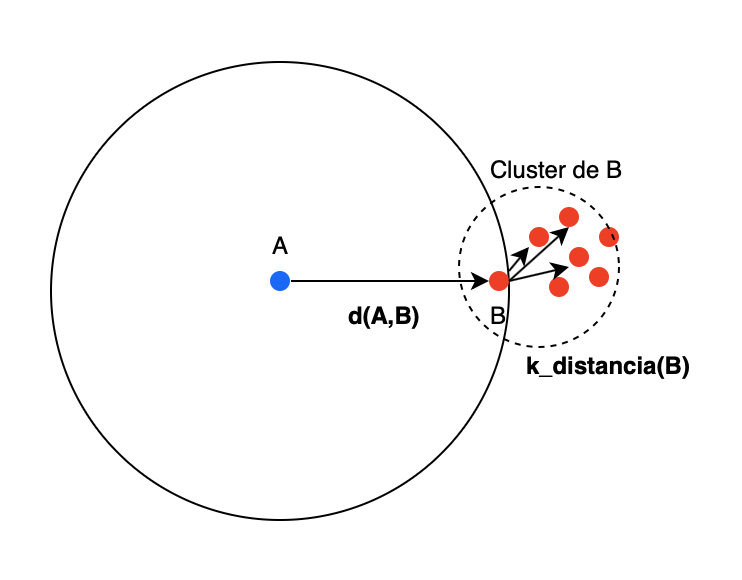
\includegraphics[width=7cm, height=5.5cm]{1}
\caption{Ejemplo del calculo de la distancia de alcance entre un punto A y un punto B}
\end{figure}
Es decir, supongamos que B pertenece a un \textit{cluster}, luego el objetivo es detectar la distancia máxima entre cualquier punto del \textit{cluster de B} con respecto al punto A, detectando de este modo a qué distancia (como máximo) se puede alcanzar el punto A.

A continuación, debemos calcular la \textbf{densidad local}. Este valor permite obtener una estimación de la distancia a partir de la cual un punto puede ser encontrado por sus vecinos \footnote{\url{https://medium.com/@doedotdev/local-outlier-factor-example-by-hand-b57cedb10bd1}}. Para ello, calculamos en primer lugar la \textbf{distancia de alcance media entre el punto A y sus \textit{k} vecinos}:
\begin{equation*}
\frac{\sum_{B \in N_{k}(A)}distancia\_alcance_{k}(A,B)}{|N_{k}(A)|}
\end{equation*}

\begin{figure}[h!]
\centering
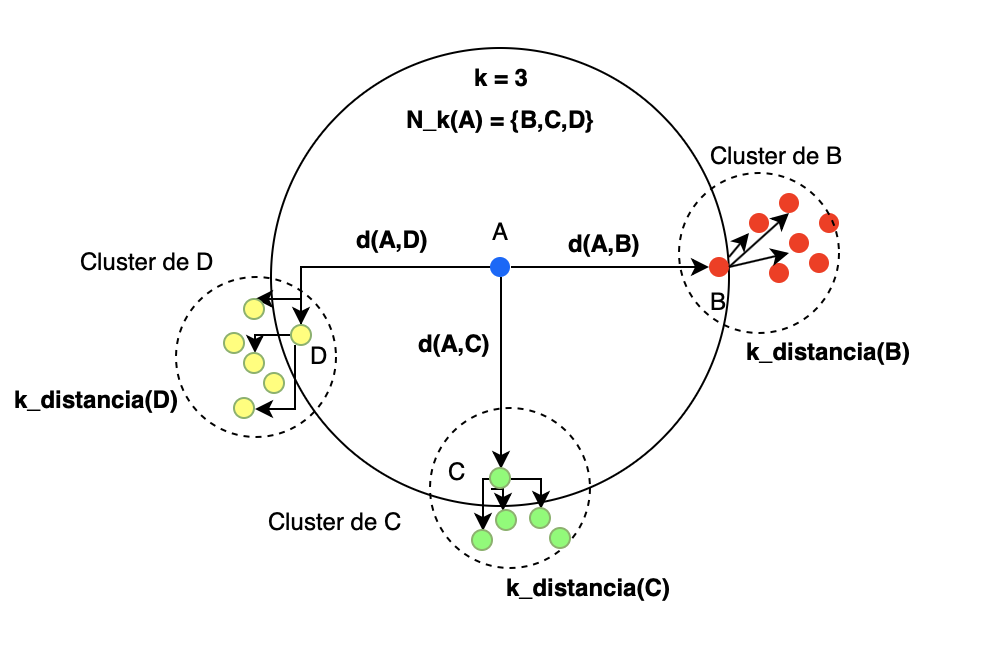
\includegraphics[width=13cm, height=9cm]{2}
\caption{Ejemplo del calculo de la densidad local entre un punto A y sus \textit{k} vecinos: \{B,C,D\}}
\end{figure}

Lo que acabamos de calcular es la \textbf{distancia media con la cual el punto A puede alcanzar cualquiera de sus vecinos}. Sin embargo, lo que queremos calcular es justo lo contrario, es decir, la \textbf{distancia desde la cual el punto A pueda ser alcanzado por sus vecinos}. Por lo tanto, la densidad local será la inversa de la media calculada:
\begin{equation*}
densidad\_local_{k}(A) = \frac{1}{\frac{\sum_{B \in N_{k}(A)}distancia\_alcance_{k}(A,B)}{|N_{k}(A)|}}
\end{equation*}

Ya tenemos la distancia media con la cual un punto A puede ser alcanzado por sus vecinos. No obstante, cada uno de los \textit{k} vecinos de A tendrá un conjunto de puntos vecinos, luego debemos calcular la \textbf{la media de densidad de cada uno de sus \textit{k} vecinos en relación con la densidad local de A}, obteniendo de este modo el \textit{Local Outliter Factor} (LOF).
\begin{equation*}
LOF_{k}(A) = \frac{\frac{\sum_{B \in N_{k}(A)}densidad\_local_{k}(B)}{|N_{k}(A)|}}{densidad\_local_{k}(A)}
\end{equation*}
\begin{itemize}
  \item LOF(k) $\sim$ 1 Implica que todos los puntos presentan la misma densidad, por lo que no se trata de un \textit{outlier}.
  \item LOF(k) < 1 implica que la densidad media local del punto A es mayor que la media de densidad local de sus \textit{k} vecinos. Al igual que en el caso anterior, no se trata de un \textit{outlier}.
  \item LOF(k) > 1 implica que la densidad media local del punto A es menor que la media de densidad local de sus \textit{k} vecinos. En este último caso, se trata de un \textit{outlier}.
\end{itemize}

\paragraph{Caso práctico: detección de \textit{outliers} con las estadísticas de tendencias en YouTube}: 
En este apartado analizaremos la detección posibles \textit{outliers} sobre vídeos etiquetados como \textbf{tendencias} en \textbf{YouTube}, concretamente en la región de Estados Unidos. \footnote{\url{https://www.kaggle.com/datasnaek/youtube-new}}

En primer lugar, importamos el fichero \textit{csv}:
\begin{Schunk}
\begin{Sinput}
> listado.videos <- read.csv("USvideos.csv")
> colnames(listado.videos)
\end{Sinput}
\begin{Soutput}
 [1] "video_id"               "trending_date"          "title"                  "channel_title"          "category_id"            "publish_time"           "tags"                   "views"                  "likes"                 
[10] "dislikes"               "comment_count"          "thumbnail_link"         "comments_disabled"      "ratings_disabled"       "video_error_or_removed" "description"           
\end{Soutput}
\end{Schunk}

El \textit{dataset} contiene un total de 16 columnas, entre las que destacan:
\begin{enumerate}
  \item Número de visualizaciones (\textit{views})
  \item Número de \textit{me gusta} (\textit{likes})
  \item Número de \textit{no me gusta} (\textit{dislikes})
  \item Número de comentarios (\textit{comment\_count})
\end{enumerate}

Para esta práctica, \textbf{analizaremos los outliers de las columnas anteriores}, realizando todas las posibles combinaciones fila-columna:
\begin{itemize}
  \item \textbf{Número de visualizaciones-número de \textit{likes}}
  \item \textbf{Número de visualizaciones-número de \textit{dislikes}}
  \item \textbf{Número de visualizaciones-número de comentarios}
\end{itemize}

Por tanto, eliminaremos el resto de columnas del \textit{dataset}:
\begin{Schunk}
\begin{Sinput}
> listado.videos2 <- listado.videos[,c(8,9,10,11)]
> head(listado.videos2)
\end{Sinput}
\begin{Soutput}
    views  likes dislikes comment_count
1  748374  57527     2966         15954
2 2418783  97185     6146         12703
3 3191434 146033     5339          8181
4  343168  10172      666          2146
5 2095731 132235     1989         17518
6  119180   9763      511          1434
\end{Soutput}
\begin{Sinput}
> # Numero de columnas
> nrow(listado.videos2)
\end{Sinput}
\begin{Soutput}
[1] 40949
\end{Soutput}
\end{Schunk}

Dado el elevado número de columnas que presenta el \textit{dataframe}, lo reducimos a 10.000:
\begin{Schunk}
\begin{Sinput}
> # Reducimos el numero de columnas a 10000
> listado.videos2 <- head(listado.videos2,10000)
\end{Sinput}
\end{Schunk}
\begin{figure}[h!]
\centering
\begin{Schunk}
\begin{Sinput}
> par(mfrow=c(2,2))
> plot(listado.videos2$views, main = "Numero de visitas", xlabel = "Fila", 
+ ylabel = "Visitas")
> plot(listado.videos2$likes, main = "Numero de \"me gusta\"", xlabel = "Fila", 
+ ylabel = "Nº \"Me gusta\"")
> plot(listado.videos2$dislikes, main = "Numero de \"no me gusta\"", xlabel = "Fila", 
+ ylabel = "Nº \"No me gusta\"")
> plot(listado.videos2$comment_count, main = "Numero de comentarios", xlabel = "Fila", 
+ ylabel = "Comentarios")
\end{Sinput}
\end{Schunk}
\includegraphics{G15-P5-039}
\caption{Columnas del dataset}
\end{figure}

Una vez reducido el tamaño del \textit{dataframe}, comenzamos con el \textbf{análisis de datos anómalos}. Para ello, \texttt{R} dispone del paquete \textit{DMwR}, el cual contiene la función \textit{lofactor}, que devuelve un vector \textbf{con el factor de \textit{outlier} de cada fila}, dado un \textit{dataframe} de entrada:
\begin{Schunk}
\begin{Sinput}
> # Importamos el paquete
> if(!require(DMwR)){
+   install.packages("DMwR")
+   require(DMwR)
+ }
\end{Sinput}
\end{Schunk}

Una vez importado, aplicamos el algoritmo \textit{LOF}. Para ello, utilizaremos la función \textit{lofactor}, pasando como parámetro el \textit{dataframe} anterior, así como el número de vecinos utilizado para el cálculo del \textit{Local Outlier Factor} (en nuestro caso elegiremos k = 5):
{\footnotesize
\begin{Schunk}
\begin{Sinput}
> # Numero de vecinos
> k = 5
> outlier.scores <- lofactor(listado.videos2, k)
> # Analicemos la salida de uno de los vectores (outliers.scores.views, por ejemplo)
> outlier.scores[1:12]
\end{Sinput}
\begin{Soutput}
 [1] 1.429558 1.065041 1.002741 1.031322 1.020761 1.019975 0.957584 1.021816 1.329381 1.072529 1.102719 1.388098
\end{Soutput}
\end{Schunk}
}
Como podemos observar, la función devuelve el grado de \textit{outlier} de cada elemento en forma de vector. Analizando el resultado, vemos que existen \textbf{datos anómalos} a lo largo del vector (aquellos cuyo factor \textit{LOF} sean mayores que 1).

A continuación, analizaremos la distribución del factor de \textit{outlier} a lo largo del \textit{dataframe}, mediante un \textbf{gráfico de densidad}:

\begin{figure}[htbp!]
\centering
\begin{Schunk}
\begin{Sinput}
> plot(density(outlier.scores), main = "Grafica de densidad", 
+ xlabel = "Fila", ylabel = "Densidad")
\end{Sinput}
\end{Schunk}
\includegraphics{G15-P5-042}
\caption{Distribucion del factor}
\end{figure}

\newpage
En conclusión, \textbf{la mayoría de los valores de cada una de las filas se concentran en torno a un valor \textit{LOF} de 1}. A continuación \textbf{reordenamos} el vector \textit{outlier} en orden ascendente, con el fin de seleccionar aquellos puntos cuyo factor \textit{LOF} sea mayor que 1 (\textit{outliers}).
Sin embargo, los factores obtenidos en el algoritmo pueden llegar a ser muy difíciles de interpretar. Por ejemplo, en un determinado \textit{dataset}, un valor de 1.1 puede ser considerado un \textit{outlier}, mientras que un factor de 2 no se considera un dato anómalo, dado que no existe un criterio específico para clasificar un punto como \textit{outlier} o no. Por ello, definimos un \textbf{factor de \textit{outlier}}, a partir del cual consideraremos a un punto como \textbf{dato anómalo} (por ejemplo, 1.2):

\begin{Schunk}
\begin{Sinput}
> # Definimos un factor de outlier
> factor_outlier <- 1.2
> # Utilizaremos la funcion order 
> # que reordena los indices del vector
> index.outliers <- order(outlier.scores[outlier.scores >= factor_outlier], decreasing = T)
> # Ejemplo
> head(index.outliers)
\end{Sinput}
\begin{Soutput}
[1]  803  774  835  804   46 1139
\end{Soutput}
\end{Schunk}

Finalmente, \textbf{representamos gráficamente los \textit{outliers}}. Para ello, crearemos un vector cuya longitud sea el número de filas, etiquetando con un \textbf{.} aquellos valores que no sean \textit{outliers}. Por otro lado, marcamos con un \textbf{+} aquellos puntos etiquetados como \textit{outliers}. A continuación, mediante la función \textit{pairs} representamos una matriz con las diferentes correlaciones, mostrando los \textit{outliers} en cada uno de ellos:
\begin{figure}[htbp!]
\centering
\begin{Schunk}
\begin{Sinput}
> n <- nrow(listado.videos2)
> # Outliers
> pch <- rep(".", n)
> # Inliers
> pch[index.outliers] <- "+"
> col <- rep("black",n)
> col[index.outliers] <- "red"
> pairs(listado.videos2, pch = pch, col = col)
\end{Sinput}
\end{Schunk}
\includegraphics{G15-P5-044}
\caption{Distribucion de los outliers con el algoritmo LOF}
\end{figure}

\newpage
\subsubsection{Extensión del algoritmo \textit{LOF}: \textit{LoOP}}
Como hemos podido comprobar, el algoritmo \textit{LOF} no proporciona la suficiente información como para clasificar un dato como \textit{outlier}. En contraposición, existe una variante del algoritmo, denominado \textit{LoOP} (\textit{Local Outlier Probabilities}), desarrollado en la universidad de Munich \footnote{\url{http://citeseerx.ist.psu.edu/viewdoc/download?doi=10.1.1.439.2035&rep=rep1&type=pdf}}. 
Mientras que el algoritmo \textit{LOF} se basa en \textbf{comparar cada una de las distancias entre un punto y sus \textit{k} vecinos}, el algoritmo \textit{LoOP} introduce un nuevo concepto para el cálculo de las distancias, \textbf{la distancia probabilística}.

Para empezar, tomamos un punto \textit{o} como valor a clasificar, así como un conjunto de puntos situados alrededor. Dicho conjunto de puntos lo denotaremos como \textit{S} (siendo \textit{S} la \textbf{distribución normal} de \textit{o}). Asumimos que \textit{o} está situado en el centro del conjunto \textit{S}.


En primer lugar, calculamos la \textbf{distancia estándar} del punto \textit{o} al resto de puntos del conjunto \textit{S} (similar al cálculo de la \textbf{desviación estándar}):
\begin{equation*}
\sigma(o,S) = \sqrt{\frac{\sum_{s \in S}{d(o,s)^2}}{|S|}}
\end{equation*}

Para el cálculo de la distancia, partimos del supuesto de que los puntos del conjunto \textit{S} se \textbf{distribuyen normalmente} alerededor de \textit{o}, por lo que debemos tener esto muy en cuenta a la hora de determinar el conjunto \textit{S}. Por ello, se pretende obtener el conjunto \textit{S} por medio del \textit{k} vecino más cercano situado alrededor de \textit{o}. De esta manera, el hecho de asumir que \textit{S} se encuentra centrado alrededor de \textit{o} es algo razonable.

Como consecuencia, definimos la \textbf{distancia probabilística} como el producto de la distancia estándar por un factor $\lambda$, obteniendo de este modo la \textbf{densidad aproximada del punto \textit{o}}:
\begin{equation*}
pdist(\lambda,o,S) = \lambda \sigma(o,S)
\end{equation*}
Donde la $\lambda$ es un \textbf{factor de normalización} (comprendido entre 1 y 3).
A continuación, calculamos el valor \textit{PLOF} (\textit{Probabilistic Local Outlier Factor}), dado el punto \textit{o} y el conjunto de los \textit{k} vecinos más cercanos a \textit{o} ($N_{k}$):
\begin{equation*}
PLOF_{\lambda,k}(o) = \frac{pdist(\lambda,o,N_{k}(o))}{E_{s \in N_{k}(o)}[pdist(\lambda,s,N_{k}(s))]} - 1
\end{equation*}
Donde E es la \textbf{estimación de la densidad de todos los puntos del conjunto \textit{S} con respecto a los \textit{k} vecinos más cercanos a \textit{o}}.
Finalmente, obtenemos el valor \textit{LoOP}:
\begin{equation*}
LoOP_{S}(o) = max(0,erf(\frac{PLOF_{\lambda,S(o)}}{\lambda \sqrt{E[(PLOF)^2]} \sqrt{2}}))
\end{equation*}
Donde $erf$ es la \textbf{función error de Gauss}. El resultado final es un valor probabilístico comprendido entre 0 y 1: un valor cercano a 0 implica que el punto se sitúa en una región densa (con un gran número de puntos alrededor), por lo que hay menos probabilidades de que se trate de un \textit{outlier}. Por el contrario, si el valor es más cercano a 1, es mucho más probable de que se trate de un \textit{outlier}.

A continuación, vamos a analizar la distribución de \textit{outliers} utilizando el mismo \textit{dataset} que en el apartado anterior. Para ello, \texttt{R} dispone del paquete \textbf{DDoutlier} \footnote{\url{https://cran.r-project.org/web/packages/DDoutlier/DDoutlier.pdf}} el cual contiene la función \textit{LOOP}, que tendrá como parámetros:
\begin{itemize}
  \item \textit{Dataframe} a analizar
  \item Número \textit{k} de vecinos (Al igual que en el ejemplo anterior, lo establecemos a 5)
  \item Factor $\lambda$ de normalización (por defecto está establecido a 3)
\end{itemize}
{\footnotesize
\begin{Schunk}
\begin{Sinput}
> # Instalamos el paquete
> if(!require(DDoutlier)){
+   install.packages("DDoutlier")
+   require(DDoutlier)
+ }
> k = 5
> outlier.scores.loop <- LOOP(listado.videos2, k = 5)
> # Analicemos el resultado
> head(outlier.scores.loop, 12)
\end{Sinput}
\begin{Soutput}
 [1] 0.345584318 0.000000000 0.000000000 0.257515866 0.010776137 0.117353546 0.130665546 0.038521712 0.431026768 0.154571492 0.009150751 0.300498501
\end{Soutput}
\end{Schunk}
}
Como podemos comprobar, el algoritmo devuelve un vector de valores comprendidos entre 0 y 1 (cuanto más cercano esté de 1, \textbf{más probabilidades habrá de que se trate de un \textit{outlier}}).
Una vez ejecutado el algoritmo, comparamos el número de \textit{outliers} obtenidos utilizando el algoritmo \textit{LOF} (para valores mayores que 1) con el número de datos anómalos obtenidos con \textit{LOOP} (valores mayores o iguales a 0.5, ya que estos tienen más posibilidades de tratarse de \textit{outliers}):
\begin{Schunk}
\begin{Sinput}
> # Total de outliers del algoritmo LOF
> length(outlier.scores[outlier.scores > 1])
\end{Sinput}
\begin{Soutput}
[1] 7024
\end{Soutput}
\begin{Sinput}
> # Total de outliers del algoritmo LoOP
> length(outlier.scores.loop[outlier.scores.loop >= 0.5])
\end{Sinput}
\begin{Soutput}
[1] 363
\end{Soutput}
\end{Schunk}

En conclusión, el número de \textit{outliers} obtenidos con el algoritmo \textit{LoOP} es \textbf{significativamente menor con respecto al número de \textit{outliers} obtenidos con el algoritmo LOF}:
\begin{figure}[htbp!]
\centering
\begin{Schunk}
\begin{Sinput}
> index.outliers.loop <- order(outlier.scores.loop[outlier.scores.loop >= 0.5], decreasing = T)
> n <- nrow(listado.videos2)
> pch <- rep(".", n)
> pch[index.outliers.loop] <- "+"
> col <- rep("black",n)
> col[index.outliers.loop] <- "red"
> pairs(listado.videos2, pch = pch, col = col)
\end{Sinput}
\end{Schunk}
\includegraphics{G15-P5-047}
\caption{Distribucion de los outliers con el algoritmo LoOP}
\end{figure}
\end{document}

\end{document}
